\documentclass[11pt,a4paper]{article}

% ===== FONT: HELVETICA =====
\usepackage[T1]{fontenc}
\usepackage[utf8]{inputenc}
\usepackage{helvet}
\renewcommand{\familydefault}{\sfdefault}

% ===== CORE PACKAGES =====
\usepackage{geometry}
\usepackage{setspace}
\usepackage{parskip}
\usepackage{enumitem}
\usepackage{float}
\usepackage{graphicx}
\usepackage{caption}
\usepackage{subcaption}

% ===== MATH =====
\usepackage{amsmath}
\usepackage{amssymb}
\usepackage{amsfonts}

% ===== TABLES =====
\usepackage{booktabs}
\usepackage{multirow}
\usepackage{array}
\usepackage{tabularx}
\usepackage{colortbl}

% ===== STYLING & BOXES =====
\usepackage{xcolor}
\usepackage[most]{tcolorbox}
\usepackage{tikz}
\usetikzlibrary{shapes,arrows.meta,positioning,fit,backgrounds,calc}

% ===== HEADERS & SECTIONS =====
\usepackage{fancyhdr}
\usepackage{titlesec}
\usepackage{tocloft}

% ===== CODE & LINKS =====
\usepackage{listings}
\usepackage{hyperref}
\usepackage{algorithm}
\usepackage{algorithmic}

% ============================================================
% COLOR PALETTE
% ============================================================
\definecolor{velblue}{RGB}{23,50,107}       % Primary deep blue
\definecolor{velaccent}{RGB}{41,98,183}     % Accent blue
\definecolor{vellight}{RGB}{232,240,254}    % Light blue bg
\definecolor{velgold}{RGB}{218,165,32}      % Gold accent
\definecolor{velgreen}{RGB}{34,120,60}      % Success green
\definecolor{velred}{RGB}{180,30,30}        % Warning red
\definecolor{velorange}{RGB}{204,102,0}     % Caution orange
\definecolor{velgray}{RGB}{245,245,248}     % Light gray bg
\definecolor{veldark}{RGB}{40,40,50}        % Dark text
\definecolor{rowalt}{RGB}{245,248,255}      % Alternating row

% ============================================================
% PAGE GEOMETRY
% ============================================================
\geometry{
    a4paper,
    left=0.75in,
    right=0.75in,
    top=0.9in,
    bottom=0.9in,
    headheight=14pt
}

\setstretch{1.12}
\setlength{\parindent}{0pt}
\setlength{\parskip}{5pt}

% ============================================================
% RUPEE SYMBOL
% ============================================================
\newcommand{\rupee}{Rs.}

% ============================================================
% HYPERLINK SETUP
% ============================================================
\hypersetup{
    colorlinks=true,
    linkcolor=velblue,
    filecolor=velaccent,
    urlcolor=velaccent,
    citecolor=velblue,
    pdftitle={Velora Mobility Optimizer -- End-Term Technical Report},
    pdfauthor={Hostel ID: 2651},
}

% ============================================================
% SECTION FORMATTING
% ============================================================
\titleformat{\section}
  {\color{velblue}\normalfont\Large\bfseries}
  {\thesection}{0.8em}{}
  [\vspace{-6pt}{\color{velblue}\titlerule[1.2pt]}]

\titleformat{\subsection}
  {\color{veldark}\normalfont\large\bfseries}
  {\thesubsection}{0.7em}{}

\titleformat{\subsubsection}
  {\color{veldark}\normalfont\normalsize\bfseries}
  {\thesubsubsection}{0.7em}{}

\titlespacing*{\section}{0pt}{14pt}{8pt}
\titlespacing*{\subsection}{0pt}{10pt}{5pt}
\titlespacing*{\subsubsection}{0pt}{8pt}{4pt}

% ============================================================
% HEADER AND FOOTER
% ============================================================
\pagestyle{fancy}
\fancyhf{}
\renewcommand{\headrulewidth}{0.6pt}
\renewcommand{\headrule}{\hbox to\headwidth{\color{velblue}\leaders\hrule height \headrulewidth\hfill}}
\fancyhead[L]{\small\color{velblue}\textbf{Velora Mobility Optimizer}}
\fancyhead[R]{\small\color{velblue}Kriti '26 --- End-Term Report}
\fancyfoot[C]{\small\thepage}

% ============================================================
% TCOLORBOX STYLES
% ============================================================
% Key insight / finding box
\newtcolorbox{insightbox}[1][Key Insight]{%
    enhanced, breakable,
    colback=vellight,
    colframe=velblue,
    coltitle=white,
    fonttitle=\bfseries,
    title={#1},
    boxrule=0.8pt,
    arc=3pt,
    left=8pt, right=8pt, top=4pt, bottom=4pt,
    toptitle=3pt, bottomtitle=3pt,
    attach boxed title to top left={yshift=-2mm, xshift=4mm},
    boxed title style={colback=velblue, arc=2pt, boxrule=0pt}
}

% Recommendation box
\newtcolorbox{recbox}[1][Recommendation]{%
    enhanced, breakable,
    colback=orange!5,
    colframe=velorange,
    coltitle=white,
    fonttitle=\bfseries,
    title={#1},
    boxrule=0.8pt,
    arc=3pt,
    left=8pt, right=8pt, top=4pt, bottom=4pt,
    toptitle=3pt, bottomtitle=3pt,
    attach boxed title to top left={yshift=-2mm, xshift=4mm},
    boxed title style={colback=velorange, arc=2pt, boxrule=0pt}
}

% Problem instance box (gray)
\newtcolorbox{instancebox}[1][Problem Instance]{%
    enhanced,
    colback=velgray,
    colframe=gray!50,
    fonttitle=\bfseries\color{veldark},
    title={#1},
    boxrule=0.6pt,
    arc=2pt,
    left=8pt, right=8pt, top=4pt, bottom=4pt
}

% Result highlight box
\newtcolorbox{resultbox}{%
    enhanced,
    colback=green!4,
    colframe=velgreen,
    boxrule=0.6pt,
    arc=2pt,
    left=8pt, right=8pt, top=6pt, bottom=6pt
}

% Violation / warning box
\newtcolorbox{warnbox}[1][Constraint Violations]{%
    enhanced,
    colback=red!3,
    colframe=velred,
    fonttitle=\bfseries\color{velred},
    title={#1},
    boxrule=0.6pt,
    arc=2pt,
    left=8pt, right=8pt, top=4pt, bottom=4pt
}

% Blue info box (hack test cases)
\newtcolorbox{hackbox}[1][]{%
    enhanced, breakable,
    colback=vellight,
    colframe=velaccent,
    fonttitle=\bfseries\color{velblue},
    title={#1},
    boxrule=0.8pt,
    arc=3pt,
    left=8pt, right=8pt, top=6pt, bottom=6pt,
    toptitle=4pt, bottomtitle=3pt,
}

% ============================================================
% TOC STYLING
% ============================================================
\renewcommand{\contentsname}{\Large\bfseries\color{velblue} Table of Contents}
\renewcommand{\cftsecfont}{\bfseries\color{velblue}}
\renewcommand{\cftsecpagefont}{\bfseries\color{velblue}}
\renewcommand{\cftsubsecfont}{\color{veldark}}
\setlength{\cftbeforesecskip}{5pt}
\setlength{\cftbeforesubsecskip}{2pt}
\renewcommand{\cftdotsep}{2}

% ============================================================
% CODE LISTING STYLE
% ============================================================
\lstset{
    basicstyle=\ttfamily\small,
    breaklines=true,
    frame=single,
    backgroundcolor=\color{velgray},
    keywordstyle=\color{velblue}\bfseries,
    commentstyle=\color{velgreen},
    stringstyle=\color{velred},
    rulecolor=\color{gray!40},
    numbers=left,
    numberstyle=\tiny\color{gray},
    numbersep=5pt
}

% ============================================================
% CUSTOM COMMANDS
% ============================================================
\newcommand{\code}[1]{\texttt{#1}}
\newcommand{\filename}[1]{\texttt{\color{velblue}#1}}
\newcommand{\statusok}{\textcolor{velgreen}{\textbf{On time}}}
\newcommand{\statustol}{\textcolor{velorange}{\textbf{Within tolerance}}}
\newcommand{\statusviol}{\textcolor{velred}{\textbf{Violated}}}
\newcommand{\saving}[1]{\textcolor{velgreen}{\textbf{#1}}}

% ============================================================
% ============================================================
% DOCUMENT START
% ============================================================
% ============================================================
\begin{document}

% ============================================================
% TITLE PAGE
% ============================================================
\begin{titlepage}
\thispagestyle{empty}
\centering

\vspace*{0.3cm}

% Top bar
\noindent\colorbox{velblue}{%
    \parbox{\dimexpr\textwidth-2\fboxsep}{%
        \centering\color{white}\large\bfseries\vspace{6pt}
        End-Term Evaluation Submission\vspace{4pt}
    }%
}

\vspace{0.2cm}
{\color{gray}\small 24th February 2026}

\vspace{1.2cm}

% Logo
\includegraphics[width=0.30\textwidth]{media/image1.png}\par

\vspace{1cm}

{\color{velblue}\rule{\textwidth}{1.5pt}}
\vspace{0.6cm}

{\Huge\bfseries\color{velblue} Velora Mobility Optimizer\par}
\vspace{0.4cm}
{\Large\color{veldark}%
A Hybrid Metaheuristic Approach for the\\[4pt]
Heterogeneous Vehicle Routing Problem\\[4pt]
with Soft Time Windows (HVRPSTW)\par}

\vspace{0.6cm}
{\color{velblue}\rule{\textwidth}{1.5pt}}

\vspace{1cm}

{\large\bfseries\color{velblue} Kriti '26 --- Optimization Problem Statement\par}

\vspace{1.2cm}

\begin{tcolorbox}[
    enhanced,
    colback=vellight,
    colframe=velblue,
    boxrule=0.8pt,
    arc=4pt,
    width=0.55\textwidth,
    halign=center,
    left=12pt, right=12pt, top=10pt, bottom=10pt
]
\centering
\begin{tabular}{rl}
\textbf{Hostel ID:} & \textbf{2651} \\[4pt]
\textbf{Submission:} & End-Term Evaluation \\[4pt]
\textbf{Domain:} & Vehicle Routing Optimization \\
\end{tabular}
\end{tcolorbox}

\vfill

{\small\color{gray} Technical Report --- \today}

\end{titlepage}

% ============================================================
% TABLE OF CONTENTS
% ============================================================
\newpage
\thispagestyle{empty}

\vspace*{-0.6cm}

\begin{tcolorbox}[
    enhanced,
    colback=vellight,
    colframe=velblue,
    boxrule=0.6pt,
    arc=3pt,
    width=\textwidth,
    halign=center,
    top=8pt, bottom=8pt
]
\centering
\textbf{\color{velblue}Repository:}\quad
\url{https://github.com/badri41/velora-mobility-optimizer}
\end{tcolorbox}

\vspace{0.4cm}

\tableofcontents

\newpage

% ============================================================
% SECTION 1: MATHEMATICAL FORMULATION
% ============================================================
\section{Mathematical Formulation}

This section presents a rigorous mathematical formulation of the Velora Mobility Optimization problem. The formulation establishes the theoretical foundation; the implemented solver relies on heuristic and meta-heuristic methods due to the problem's NP-hard computational complexity.

\subsection{Problem Structure and Graph Model}

We model the system as a directed graph $G = (V, A)$, where:
\[
V = D \;\cup\; P \;\cup\; \{c\}.
\]

\begin{instancebox}[Node Sets]
\begin{itemize}[nosep, leftmargin=1.2em]
    \item $D = \{d_1, d_2, \dots, d_m\}$\,---\,vehicle start locations (depots)
    \item $P = \{1, 2, \dots, n\}$\,---\,employee pickup locations
    \item $c$\,---\,single common drop-off location (office/campus)
\end{itemize}
\end{instancebox}

Each employee request $i \in P$ consists of a pickup at node $i$ and a drop-off at node $c$.

Let $K$ denote the set of \textbf{heterogeneous vehicles} \cite{dondo2007,golden2008}. Each vehicle $k \in K$:
\begin{itemize}[nosep, leftmargin=1.2em]
    \item starts from depot $d(k) \in D$, with capacity $Q_k$,
    \item incurs cost $C_k$ per kilometre, available from time $A_k$.
\end{itemize}

For each arc $(u,v) \in A$, let $d_{uv}$ be the travel distance and $\tau_{uv} = d_{uv}/v$ be the travel time (constant average speed). Each employee $i$ has a soft time window $[E_i, L_i]$ for arrival at $c$ and a priority level $P_i \in \{1,2,3,4,5\}$ (lower = higher priority).

\subsection{Decision Variables}

\begin{itemize}[nosep, leftmargin=1.2em]
    \item $x_{uv}^k \in \{0,1\}$: equals 1 if vehicle $k$ traverses arc $(u,v)$
    \item $t_u^k \ge 0$: arrival time of vehicle $k$ at node $u$
    \item $q_u^k \ge 0$: passengers onboard vehicle $k$ after leaving node $u$
\end{itemize}

\subsection{Objective Function}

Minimize total operational cost plus penalties for late arrivals and unassigned employees:

\begin{equation}
\min \; Z = w_c \cdot Z_{\text{dist}} + w_t \cdot Z_{\text{time}} +  Z_{\text{late}} + Z_{\text{unassigned}}
\end{equation}

\subsubsection{Operating Cost}
\begin{equation}
Z_{\text{dist}} =
\sum_{k \in K} \sum_{(u,v)\in A}
C_k \, d_{uv} \, x_{uv}^k
\end{equation}

\subsubsection{Operating Time}
\begin{equation}
Z_{\text{time}} = \sum_{k \in K} T_k, \qquad
T_k = \sum_{(u,v) \in A} \tau_{uv} \cdot x_{uv}^k
\end{equation}
where $T_k$ is the total travel time for vehicle $k$ across all path segments.

\subsubsection{Lateness Penalty (Two-Tier Structure)}

For each employee $i$, let $t_c^k$ denote the arrival time at the office by their assigned vehicle $k$, and $f(P_i)$ the priority-based tolerance (grace period) in minutes:

\begin{equation}
\text{Penalty}_i = 
\begin{cases}
0 & \text{if } t_c^k \leq L_i + f(P_i) \\[4pt]
(t_c^k - L_i - f(P_i)) \cdot M \cdot w(P_i) & \text{if } t_c^k > L_i + f(P_i)
\end{cases}
\end{equation}

\begin{insightbox}[Tolerance Configuration]
\begin{tabular}{lccccc}
\toprule
\textbf{Priority} & P1 & P2 & P3 & P4 & P5 \\
\midrule
\textbf{Tolerance $f(P_i)$} & 5\,min & 10\,min & 15\,min & 20\,min & 30\,min \\
\textbf{Weight $w(P_i)$} & 5 & 4 & 3 & 2 & 1 \\
\bottomrule
\end{tabular}

\vspace{4pt}
\textbf{No penalty} is incurred as long as the employee arrives within $L_i + f(P_i)$. Only arrivals \emph{exceeding} this tolerance incur the severe multiplier $M = 1000$.
\end{insightbox}

Total lateness penalty:
\begin{equation}
Z_{\text{penalty}} = \sum_{i\in P} \text{Penalty}_i
\end{equation}

\subsubsection{Unassigned Penalty}
\begin{equation}
Z_{\text{unassigned}} = M \cdot |\{i \in P : i \text{ unassigned}\}|,\qquad M \gg 1
\end{equation}

\subsection{Constraints}

\begin{minipage}[t]{0.48\textwidth}
\textbf{Pickup Assignment}\\
Each employee served by at most one vehicle:
\begin{equation}
\sum_{k\in K}\sum_{v\in V} x_{iv}^k \le 1 \;\;\forall i \in P
\end{equation}

\textbf{Flow Conservation}\\
For each vehicle $k$:
\begin{equation}
\sum_{v} x_{uv}^k - \sum_{v} x_{vu}^k = 0
\end{equation}
$\forall u \in V \setminus \{d(k), c\}$.

\textbf{Route Structure}\\
Each vehicle starts from exactly one depot $d(k)$ and ends at the common drop node $c$.
\end{minipage}
\hfill
\begin{minipage}[t]{0.48\textwidth}
\textbf{Capacity Constraints}
\begin{align}
0 \le q_u^k &\le Q_k \;\;\forall u,k \\
q_v^k &\ge q_u^k + \delta(v) - (1{-}x_{uv}^k)M'
\end{align}
where $\delta(v)=1$ for pickup nodes.

\textbf{Time Propagation}
\begin{equation}
t_v^k \ge t_u^k + \tau_{uv} - (1{-}x_{uv}^k)M''
\end{equation}

\textbf{Vehicle Availability}
\begin{equation}
t_{d(k)}^k \ge A_k \;\;\forall k\in K
\end{equation}
\end{minipage}

\vspace{8pt}

\textbf{Pickup Time Window:}
\begin{equation}
t_i^k \ge E_i - (1 - \sum_{v \in V} x_{iv}^k) \cdot M \qquad \forall i \in P,\; \forall k \in K
\end{equation}

\subsection{Distance Calculation}

The system uses adjusted Haversine distance to approximate road distance:
\begin{equation}
D_{\text{road}} \approx 1.4 \times D_{\text{haversine}}
\end{equation}
The $1.4\times$ multiplier accounts for urban road network geometry (roads are 30--50\% longer than straight-line distances).

% ============================================================
% SECTION 2: ALGORITHM DESIGN
% ============================================================
\section{Algorithm Design (Implemented Hybrid)}

The solver implements a two-phase hybrid approach combining a constructive heuristic with simulated annealing metaheuristic optimization.

\subsection{Phase 1: Multi-Start Constructive Insertion}

Requests are sorted by priority and time urgency; across multiple restarts, the order is perturbed to diversify constructions \cite{solomon1987,cordeau2002}.

For vehicle $k$ with route $R_k=(v_0,\dots,v_m)$ and request $u$, evaluate insertion indices $(i,j)$ with $i<j$ and minimize \cite{solomon1987}:
\begin{equation}
\Delta(u,k,i,j)= w_c\,\Delta\text{CTC}(u,k,i,j)+ w_t\,\Delta\text{Time}(u,k,i,j) + \Delta\text{Penalty}(u,k,i,j)
\end{equation}

\subsection{Phase 2: Simulated Annealing (SA)}

Simulated Annealing is a probabilistic metaheuristic for global optimization \cite{kirkpatrick1983}. Given current solution $S$ and neighbor $S'$, define $\Delta E = Z(S')-Z(S)$:

\begin{equation}
\Pr(\text{accept})=
\begin{cases}
1 & \Delta E<0\\
\exp(-\Delta E/T) & \Delta E\ge 0
\end{cases}
\end{equation}

\begin{insightbox}[SA Hyperparameters]
\begin{tabular}{llp{7cm}}
\toprule
\textbf{Parameter} & \textbf{Value} & \textbf{Rationale} \\
\midrule
$T_0$ & $\min(0.3 \times Z_{\text{init}},\; 1000)$ & Adaptive to instance scale; cap prevents accepting wildly worse solutions in penalty-heavy instances \\
$\alpha$ & 0.99 & Geometric cooling: $T_{r+1} = \alpha\, T_r$ \\
$T_{\min}$ & 1.0 & Floor temperature where SA terminates \\
Max no-improve & $1500 / \text{scale}$ & Patience scales inversely with route complexity \\
Wall-clock limit & 24\,s & Hard deadline for deployment constraints \\
\bottomrule
\end{tabular}
\end{insightbox}

\subsubsection{Neighborhood Operators}

The SA phase employs \textbf{five weighted operators} selected via discrete probability distribution:

\begin{table}[H]
\centering
\caption{SA neighborhood operators and selection weights}
\label{tab:operators}
\begin{tabular}{llcc}
\toprule
\textbf{Operator} & \textbf{Description} & \textbf{Weight} & \textbf{Complexity} \\
\midrule
\rowcolor{rowalt}
Greedy Relocate   & Try ALL routes for best insertion of a random request  & 25 & $O(N \cdot V)$ \\
Intra-Route Relocate & Or-opt style: move a request within the same route & 30 & $O(N)$ \\
\rowcolor{rowalt}
2-Opt             & Reverse a segment within a route                       & 20 & $O(N)$ \\
Exchange          & Swap requests between two different routes              & 15 & $O(1)$ \\
\rowcolor{rowalt}
Random Relocate   & Move a request to a random position in a random route   & 10 & $O(1)$ \\
\bottomrule
\end{tabular}
\end{table}

\subsection{Time Complexity}

\[
T = \underbrace{O(N \log N)}_{\text{sort}}
  + \underbrace{O(V^2)}_{\text{exact search}}
  + \underbrace{O\!\left(\frac{R \cdot N^3}{V}\right)}_{\text{subsampled search}}
  + \underbrace{O\!\left(I \cdot \frac{N^2}{V^2}\right)}_{\text{simulated annealing}}
  + \underbrace{O(N^2)}_{\text{distance matrix}}
\]

\noindent where $R = \max\!\bigl(1,\;\min\!\bigl(10,\;\lfloor 50 / \lceil 2N/V \rceil\rfloor\bigr)\bigr)$ is the number of construction restarts, and $I$ is the number of SA iterations (bounded by a 24-second wall-clock deadline).

\begin{resultbox}
For $N \gg V$:\quad
$\displaystyle\boxed{O\!\left(\frac{N^3}{V}\right)}$
\end{resultbox}

% ============================================================
% SECTION 3: SYSTEM ARCHITECTURE
% ============================================================
\newpage
\section{System Architecture}
\label{sec:architecture}

The Velora Mobility Optimizer implements a complete \textbf{10-stage data flow pipeline} spanning three layers: Frontend (React.js + Vite), Backend (Express.js), and Solver (C++17).

\subsection{Pipeline Architecture}

\begin{figure}[H]
\centering
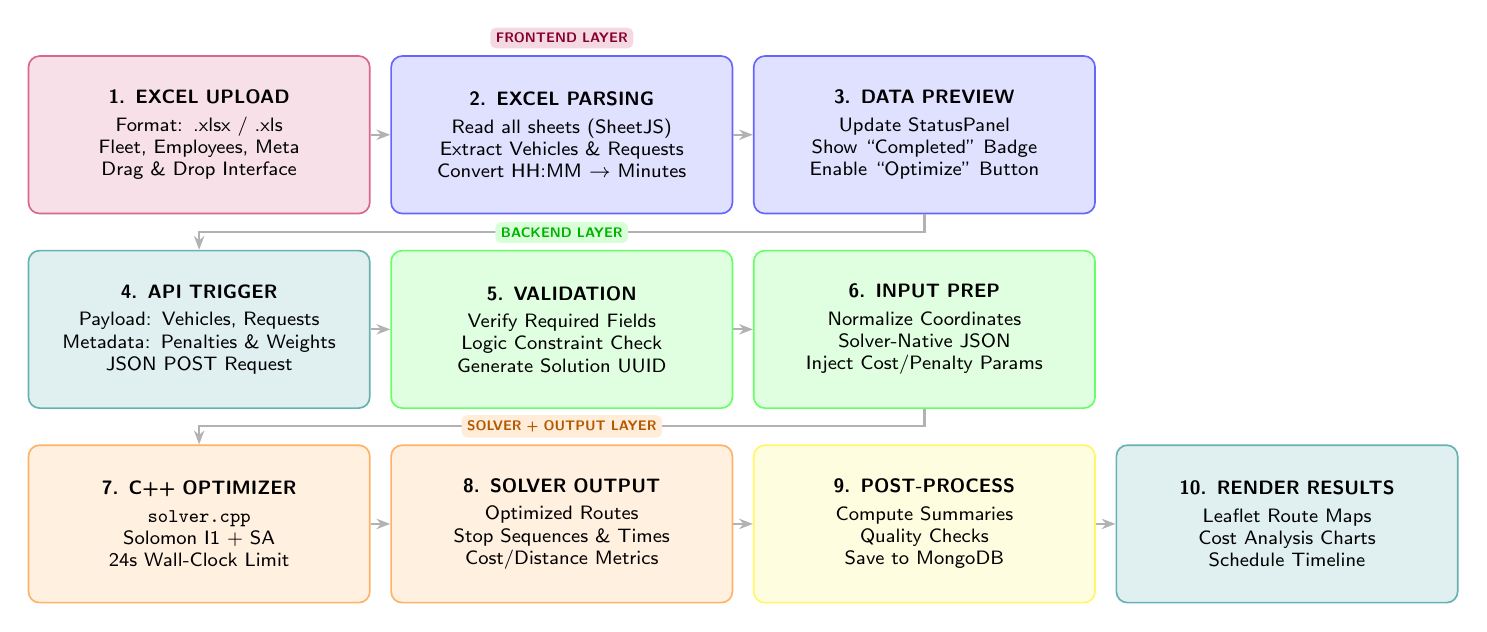
\begin{tikzpicture}[
    node distance=0.35cm,
    stage/.style={rectangle, draw=#1!60, fill=#1!12, text width=4.1cm, text centered, minimum height=2cm, rounded corners=4pt, font=\scriptsize, line width=0.6pt},
    lbl/.style={font=\tiny\bfseries, inner sep=2pt, rounded corners=2pt},
    arrow/.style={-{Stealth[length=5pt]}, thick, color=gray!60}
]
    % Row 1: Frontend (1-3)
    \node[stage=purple] (s1) {\textbf{1. EXCEL UPLOAD}\\[2pt]Format: .xlsx / .xls\\Fleet, Employees, Meta\\Drag \& Drop Interface};
    
    \node[stage=blue, right=0.25cm of s1] (s2) {\textbf{2. EXCEL PARSING}\\[2pt]Read all sheets (SheetJS)\\Extract Vehicles \& Requests\\Convert HH:MM $\to$ Minutes};
    
    \node[stage=blue, right=0.25cm of s2] (s3) {\textbf{3. DATA PREVIEW}\\[2pt]Update StatusPanel\\Show ``Completed'' Badge\\Enable ``Optimize'' Button};
    
    % Row 2: Backend (4-6)
    \node[stage=teal, below=0.45cm of s1] (s4) {\textbf{4. API TRIGGER}\\[2pt]Payload: Vehicles, Requests\\Metadata: Penalties \& Weights\\JSON POST Request};
    
    \node[stage=green, right=0.25cm of s4] (s5) {\textbf{5. VALIDATION}\\[2pt]Verify Required Fields\\Logic Constraint Check\\Generate Solution UUID};
    
    \node[stage=green, right=0.25cm of s5] (s6) {\textbf{6. INPUT PREP}\\[2pt]Normalize Coordinates\\Solver-Native JSON\\Inject Cost/Penalty Params};
    
    % Row 3: Solver + Output (7-10)
    \node[stage=orange, below=0.45cm of s4] (s7) {\textbf{7. C++ OPTIMIZER}\\[2pt]\texttt{solver.cpp}\\Solomon I1 + SA\\24s Wall-Clock Limit};
    
    \node[stage=orange, right=0.25cm of s7] (s8) {\textbf{8. SOLVER OUTPUT}\\[2pt]Optimized Routes\\Stop Sequences \& Times\\Cost/Distance Metrics};
    
    \node[stage=yellow, right=0.25cm of s8] (s9) {\textbf{9. POST-PROCESS}\\[2pt]Compute Summaries\\Quality Checks\\Save to MongoDB};
    
    \node[stage=teal, right=0.25cm of s9] (s10) {\textbf{10. RENDER RESULTS}\\[2pt]Leaflet Route Maps\\Cost Analysis Charts\\Schedule Timeline};
    
    % Arrows
    \draw[arrow] (s1) -- (s2);
    \draw[arrow] (s2) -- (s3);
    \draw[arrow] (s3.south) -- ++(0,-0.22) -| (s4.north);
    \draw[arrow] (s4) -- (s5);
    \draw[arrow] (s5) -- (s6);
    \draw[arrow] (s6.south) -- ++(0,-0.22) -| (s7.north);
    \draw[arrow] (s7) -- (s8);
    \draw[arrow] (s8) -- (s9);
    \draw[arrow] (s9) -- (s10);
    
    % Layer labels
    \node[lbl, fill=purple!15, above=0.08cm of s2] {\color{purple!70!black}FRONTEND LAYER};
    \node[lbl, fill=green!15, above=0.08cm of s5] {\color{green!70!black}BACKEND LAYER};
    \node[lbl, fill=orange!15, above=0.08cm of s8] {\color{orange!70!black}SOLVER + OUTPUT LAYER};
\end{tikzpicture}
\caption{10-Stage System Architecture Data Flow Pipeline}
\label{fig:dataflow}
\end{figure}

\subsection{Component Architecture}

\begin{figure}[H]
\centering
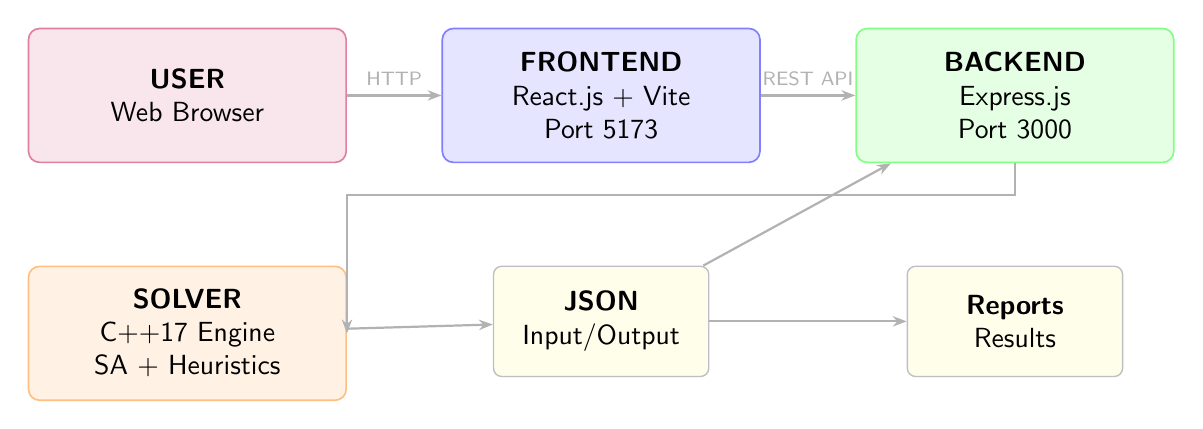
\begin{tikzpicture}[
    node distance=0.8cm,
    comp/.style={rectangle, draw=#1!50, fill=#1!10, text width=3.8cm, text centered, minimum height=1.7cm, rounded corners=4pt, line width=0.6pt},
    data/.style={rectangle, draw=gray!50, fill=yellow!8, text width=2.5cm, text centered, minimum height=1.4cm, rounded corners=3pt, line width=0.5pt},
    arrow/.style={-{Stealth[length=5pt]}, thick, color=gray!60}
]
    \node[comp=purple] (user) {\textbf{USER}\\Web Browser};
    \node[comp=blue, right=1.2cm of user] (frontend) {\textbf{FRONTEND}\\React.js + Vite\\Port 5173};
    \node[comp=green, right=1.2cm of frontend] (backend) {\textbf{BACKEND}\\Express.js\\Port 3000};
    \node[comp=orange, below=1.3cm of user] (solver) {\textbf{SOLVER}\\C++17 Engine\\SA + Heuristics};
    \node[data, below=1.3cm of frontend] (json) {\textbf{JSON}\\Input/Output};
    \node[data, below=1.3cm of backend] (report) {\textbf{Reports}\\Results};
    
    \draw[arrow] (user) -- node[above, font=\scriptsize] {HTTP} (frontend);
    \draw[arrow] (frontend) -- node[above, font=\scriptsize] {REST API} (backend);
    \draw[arrow] (backend.south) -- ++(0,-0.4) -| (solver.east);
    \draw[arrow] (solver) -- (json);
    \draw[arrow] (json) -- (backend);
    \draw[arrow] (json) -- (report);
\end{tikzpicture}
\caption{High-Level Component Architecture}
\label{fig:arch}
\end{figure}

% ============================================================
% SECTION 4: EXPERIMENTAL RESULTS
% ============================================================
\newpage
\section{Experimental Results}

We evaluated the system on four test cases (TC01--TC04) of increasing complexity. Each test case was run in two configurations: (1)~with penalty weights set to zero (pure cost optimization), and (2)~with non-zero penalties (constraint-aware optimization for TC04). The following metrics are from the solver-generated reports.

\subsection{Results Overview}

\begin{table}[H]
\centering
\caption{Cross--test-case performance comparison}
\label{tab:overview}
\begin{tabular}{lcccccc}
\toprule
\textbf{Test Case} & \textbf{Employees} & \textbf{Vehicles} & \textbf{Cost Saving} & \textbf{Time Saving} & \textbf{Routes Used} & \textbf{Global Cost} \\
\midrule
\rowcolor{rowalt}
TC01 & 8  & 3 & \saving{85.0\%} & \saving{37.6\%} & 2 / 3 & 415.24 \\
TC02 & 12 & 5 & \saving{85.1\%} & \saving{39.4\%} & 3 / 5 & 612.15 \\
\rowcolor{rowalt}
TC03 & 15 & 6 & \saving{85.3\%} & \saving{52.9\%} & 3 / 6 & 714.19 \\
TC04 & 10 & 4 & \saving{58.2\%} & \saving{27.6\%} & 4 / 4 & 1,556,091 \\
\bottomrule
\end{tabular}
\end{table}

\begin{insightbox}[Overall Trend]
All test cases achieve \textbf{$>$\!58\% cost reduction} over individual-trip baselines. TC01--TC03 (penalties at zero) reach $\sim$85\% savings by aggressively consolidating routes, while TC04 (with active penalties) trades some cost efficiency for constraint compliance. The high global cost in TC04 stems from a single structurally infeasible employee (E10).
\end{insightbox}

% ============================================================
% TC01
% ============================================================
\subsection{Test Case 01 --- 8 Employees, 3 Vehicles}

\begin{instancebox}
8 employees transported to a common office using 3 heterogeneous vehicles (1 premium electric, 1 normal petrol, 1 normal diesel van). Objective weights: Cost 70\% / Time 30\%. All soft-constraint penalty weights set to zero.
\end{instancebox}

\subsubsection{Solution Summary}

\begin{minipage}[t]{0.48\textwidth}
\begin{table}[H]
\centering
\begin{tabular}{lcc}
\toprule
\textbf{Metric} & \textbf{Optimized} & \textbf{Baseline} \\
\midrule
\rowcolor{rowalt}
Cost (\rupee) & 479.47 & 3,200.00 \\
Time (min) & 265.36 & 425.00 \\
\rowcolor{rowalt}
Distance (km) & 42.20 & --- \\
Vehicles Used & 2 / 3 & --- \\
\rowcolor{rowalt}
Unassigned & 0 & --- \\
\bottomrule
\end{tabular}
\end{table}
\end{minipage}
\hfill
\begin{minipage}[t]{0.48\textwidth}
\begin{table}[H]
\centering
\begin{tabular}{llcc}
\toprule
\textbf{Veh.} & \textbf{Type} & \textbf{Emp.} & \textbf{Cost} \\
\midrule
\rowcolor{rowalt}
V01 & Premium (Elec.) & 4 & \rupee\,278.20 \\
V02 & Normal (Petrol) & 4 & \rupee\,201.28 \\
\rowcolor{rowalt}
V03 & Van (Diesel) & 0 & \rupee\,0 \\
\bottomrule
\end{tabular}
\end{table}
\end{minipage}

\vspace{4pt}
\textbf{Savings:} \saving{85.0\%} cost reduction, \saving{37.6\%} time reduction.\quad Global cost: 415.24.

\subsubsection{Constraint Violations (4 of 8 Employees)}

\begin{warnbox}
\small
\begin{tabular}{>{\bfseries}l c p{8.5cm}}
\toprule
\textbf{Employee} & \textbf{Pri.} & \textbf{Issue} \\
\midrule
\rowcolor{red!4}
E06 & P1 & Pickup 23\,min late (09:38 vs 09:20); sharing violated (3 pax, limit 1) \\
E01 & P1 & Dropoff 41\,min late (10:16 vs 09:35); wrong vehicle (normal vs premium); sharing (4 vs 1) \\
\rowcolor{red!4}
E04 & P2 & Pickup 11\,min late; dropoff 21\,min late; sharing (4 vs 2) \\
E02 & P2 & Dropoff 6\,min late (10:16 vs 10:10); sharing (4 vs 2) \\
\bottomrule
\end{tabular}

\vspace{4pt}
E03, E07: minor vehicle preference mismatches but on time.\; E05, E08: no violations.
\end{warnbox}

\begin{recbox}
With all penalty weights at zero, the solver optimizes purely on cost/time with no disincentive for constraint violations. Setting \code{lateArrivalPenaltyPerMin} $\geq$ 50, \code{sharingViolationPenalty} $\geq$ 500, and \code{vehiclePrefViolationPenalty} $\geq$ 200 would yield more feasible solutions at modest cost increase.
\end{recbox}

\begin{figure}[H]
    \centering
    
\includegraphics[width=0.72\textwidth]{tc01_convergence.png}
    \caption{SA Convergence --- TC01: Quick convergence within $\sim$475 iterations due to small instance size.}
    \label{fig:conv-tc01}
\end{figure}

% ============================================================
% TC02
% ============================================================
\subsection{Test Case 02 --- 12 Employees, 5 Vehicles}

\begin{instancebox}
12 employees, 5 heterogeneous vehicles (2 premium electric, 1 normal petrol, 1 diesel van, 1 two-wheeler). Objective weights: Cost 65\% / Time 35\%. All soft-constraint penalties at zero except \code{unassignedPenalty} = 100{,}000.
\end{instancebox}

\subsubsection{Solution Summary}

\begin{minipage}[t]{0.48\textwidth}
\begin{table}[H]
\centering
\begin{tabular}{lcc}
\toprule
\textbf{Metric} & \textbf{Optimized} & \textbf{Baseline} \\
\midrule
\rowcolor{rowalt}
Cost (\rupee) & 734.56 & 4,945.00 \\
Time (min) & 384.81 & 635.00 \\
\rowcolor{rowalt}
Distance (km) & 72.91 & --- \\
Vehicles Used & 3 / 5 & --- \\
\rowcolor{rowalt}
Penalty Cost & 0 & --- \\
\bottomrule
\end{tabular}
\end{table}
\end{minipage}
\hfill
\begin{minipage}[t]{0.48\textwidth}
\begin{table}[H]
\centering
\begin{tabular}{llrc}
\toprule
\textbf{Veh.} & \textbf{Type} & \textbf{Dist.} & \textbf{Cost} \\
\midrule
\rowcolor{rowalt}
V01 & Premium (Elec.) & 32.9\,km & \rupee\,329 \\
V04 & Premium (Elec.) & 28.5\,km & \rupee\,313 \\
\rowcolor{rowalt}
V05 & 2W (Petrol) & 11.5\,km & \rupee\,92 \\
V02, V03 & \textit{Unused} & 0\,km & \rupee\,0 \\
\bottomrule
\end{tabular}
\end{table}
\end{minipage}

\vspace{4pt}
\textbf{Savings:} \saving{85.1\%} cost, \saving{39.4\%} time.\quad Global cost: 612.15.

\subsubsection{Constraint Violations (5 of 12 Employees)}

\begin{warnbox}
\small
\begin{tabular}{>{\bfseries}l c p{8.5cm}}
\toprule
\textbf{Employee} & \textbf{Pri.} & \textbf{Issue} \\
\midrule
\rowcolor{red!4}
E01 & P1 & Pickup 61\,min late (10:21 vs 09:20); dropoff violated; sharing (3 vs 1) \\
E06 & P1 & Pickup 48\,min late (09:53 vs 09:05); dropoff violated; sharing (3 vs 1) \\
\rowcolor{red!4}
E12 & P1 & Pickup 28\,min late (09:48 vs 09:20); dropoff violated; sharing (3 vs 1) \\
E02 & P2 & Pickup 25\,min late; dropoff violated; sharing (3 vs 2) \\
\rowcolor{red!4}
E04 & P2 & Pickup 20\,min late; dropoff violated; sharing (3 vs 2) \\
\bottomrule
\end{tabular}

\vspace{4pt}
On-time: E03, E05, E07, E08, E09, E10, E11 (7/12). Minor sharing/pref mismatches for E03, E07, E10, E11.
\end{warnbox}

\begin{recbox}
All three P1 employees are violated. V04 carries 6 employees sequentially with up to 3 concurrent. Setting non-zero penalties would force utilization of V02/V03 and improve compliance.
\end{recbox}

\begin{figure}[H]
    \centering
    
\includegraphics[width=0.72\textwidth]{tc02_convergence.png}
    \caption{SA Convergence --- TC02: Multiple improvement stages, last improvement at $\sim$1351 iterations.}
    \label{fig:conv-tc02}
\end{figure}

% ============================================================
% TC03
% ============================================================
\newpage
\subsection{Test Case 03 --- 15 Employees, 6 Vehicles}

\begin{instancebox}
15 employees, 6 heterogeneous vehicles (2 premium electric, 1 normal petrol, 1 diesel van, 1 two-wheeler, 1 extra petrol). Objective weights: Cost 60\% / Time 40\%. All soft-constraint penalties at zero except \code{unassignedPenalty} = 100{,}000. Tighter tolerance: P1=5, P2=8, P3=12, P4=18, P5=30\,min.
\end{instancebox}

\subsubsection{Solution Summary}

\begin{minipage}[t]{0.48\textwidth}
\begin{table}[H]
\centering
\begin{tabular}{lcc}
\toprule
\textbf{Metric} & \textbf{Optimized} & \textbf{Baseline} \\
\midrule
\rowcolor{rowalt}
Cost (\rupee) & 947.04 & 6,450.00 \\
Time (min) & 364.92 & 775.00 \\
\rowcolor{rowalt}
Distance (km) & 77.66 & --- \\
Vehicles Used & 3 / 6 & --- \\
\rowcolor{rowalt}
Penalty Cost & 0 & --- \\
\bottomrule
\end{tabular}
\end{table}
\end{minipage}
\hfill
\begin{minipage}[t]{0.48\textwidth}
\begin{table}[H]
\centering
\small
\begin{tabular}{llrc}
\toprule
\textbf{Veh.} & \textbf{Employees} & \textbf{Dist.} & \textbf{Cost} \\
\midrule
\rowcolor{rowalt}
V01 & E08,07,04,14,09,06,15,11 & 49.5\,km & \rupee\,495 \\
V04 & E01,02,03,05,12,13 & 20.6\,km & \rupee\,392 \\
\rowcolor{rowalt}
V05 & E10 & 7.6\,km & \rupee\,60 \\
\multicolumn{4}{l}{\textit{V02, V03, V06 unused}} \\
\bottomrule
\end{tabular}
\end{table}
\end{minipage}

\vspace{4pt}
\textbf{Savings:} \saving{85.3\%} cost, \saving{52.9\%} time.\quad Global cost: 714.19.

\subsubsection{Constraint Violations (8 of 15 Employees)}

\begin{warnbox}
\small
\begin{tabular}{>{\bfseries}l c p{8.5cm}}
\toprule
\textbf{Employee} & \textbf{Pri.} & \textbf{Issue} \\
\midrule
\rowcolor{red!4}
E07 & P1 & Pickup 6\,min late (09:11 vs 09:05); sharing (2 vs 1) \\
E01 & P1 & Pickup 18\,min late (09:23 vs 09:05); wanted premium, got van; sharing (6 vs 1) \\
\rowcolor{red!4}
E02 & P1 & Van instead of premium; sharing (6 vs 1); timing violated \\
E13 & P1 & Van instead of premium; sharing (6 vs 1); timing violated \\
\rowcolor{red!4}
E06 & P2 & Pickup 36\,min late (10:29 vs 09:53); sharing (3 vs 2) \\
E11 & P2 & Pickup 36\,min late (10:34 vs 09:58); sharing (3 vs 2) \\
\rowcolor{red!4}
E15 & P2 & Pickup 37\,min late; pref violated (normal$\to$premium); sharing (3 vs 2) \\
E04 & P3 & Dropoff $\sim$2\,min late; pref violated (normal$\to$premium) \\
\bottomrule
\end{tabular}

\vspace{4pt}
On-time: E08, E09, E10, E14 (4/15). Half the fleet (V02, V03, V06) is idle while V01 serves 8 employees.
\end{warnbox}

\begin{insightbox}[Critical Finding]
All 4 priority-1 employees are violated. V01 is overloaded with 8 employees (capacity 3) while 3 vehicles sit idle, demonstrating extreme over-consolidation when penalty weights are zero. The solver has no incentive to respect sharing limits or vehicle preferences.
\end{insightbox}

\begin{figure}[H]
    \centering
    
\includegraphics[width=0.72\textwidth]{tc03_convergence.png}
    \caption{SA Convergence --- TC03: Steady improvement over $\sim$7200 iterations. Largest instance benefits most from extended SA exploration.}
    \label{fig:conv-tc03}
\end{figure}

% ============================================================
% TC04 - WITH PENALTIES
% ============================================================
\newpage
\subsection{Test Case 04 --- 10 Employees, 4 Vehicles (Penalties Active)}

\begin{instancebox}
10 employees, 4 heterogeneous vehicles (2 premium electric, 1 normal petrol, 1 normal diesel van). Objective weights: Cost 70\% / Time 30\%. \textbf{Priority-based delay tolerances active} (P1: 5\,min $\to$ P5: 30\,min) with severe penalty multiplier $M = 1000$.
\end{instancebox}

\subsubsection{Vehicle Fleet}

\begin{table}[H]
\centering
\begin{tabular}{lccccl}
\toprule
\textbf{Vehicle} & \textbf{Category} & \textbf{Capacity} & \textbf{Cost/km (\rupee)} & \textbf{Speed} & \textbf{Fuel} \\
\midrule
\rowcolor{rowalt}
V01 & Premium & 2 & 10 & 30\,km/h & Electric \\
V02 & Premium & 2 & 11 & 28\,km/h & Electric \\
\rowcolor{rowalt}
V03 & Normal  & 4 & 14 & 35\,km/h & Petrol \\
V04 & Normal (Van) & 6 & 18 & 32\,km/h & Diesel \\
\bottomrule
\end{tabular}
\caption{TC04 vehicle fleet specification}
\label{tab:tc04-fleet}
\end{table}

\subsubsection{Solution Summary}

\begin{table}[H]
\centering
\begin{tabular}{lccc}
\toprule
\textbf{Metric} & \textbf{Optimized} & \textbf{Baseline} & \textbf{Savings} \\
\midrule
\rowcolor{rowalt}
Monetary Cost (\rupee) & 1,846.94 & 4,420.00 & \saving{58.2\%} \\
Total Time (min) & 351.04 & 485.00 & \saving{27.6\%} \\
\rowcolor{rowalt}
Vehicles Used & 4 & 10 (individual) & \saving{60\% fewer} \\
Total Distance & 150.60\,km & --- & --- \\
\rowcolor{rowalt}
Penalty Cost & \rupee\,1,554,692.86 & --- & --- \\
\bottomrule
\end{tabular}
\end{table}

10 individual trips consolidated into 4 shared routes. The entire penalty stems from one outlier (E10).

\subsubsection{Route Details}

\textbf{Route 1 --- V01 (Premium, Electric) $|$ 5 employees $|$ 57.56\,km}

\begin{table}[H]
\centering
\begin{tabular}{llllc}
\toprule
\textbf{Emp.} & \textbf{Pri.} & \textbf{Pickup} & \textbf{Dropoff} & \textbf{Status} \\
\midrule
\rowcolor{rowalt}
E01 & P1 & 08:10 & 08:24 & \statusok \\
E03 & P1 & 08:40 & 08:54 & \statusok \\
\rowcolor{rowalt}
E05 & P2 & 09:09 & 09:28 & \statusok \\
E06 & P2 & 09:11 & 09:28 & \statusok \\
\rowcolor{rowalt}
E09 & P4 & 09:44 & 10:03 & \statusok \\
\bottomrule
\end{tabular}
\end{table}
Cost: \rupee\,575.63 vs baseline \rupee\,2,095 $\rightarrow$ \saving{72.5\% savings}. E05 and E06 share the vehicle simultaneously (both allow sharing limit of 2).

\vspace{6pt}
\textbf{Route 2 --- V02 (Premium, Electric) $|$ 2 employees $|$ 21.89\,km}

\begin{table}[H]
\centering
\begin{tabular}{llllc}
\toprule
\textbf{Emp.} & \textbf{Pri.} & \textbf{Pickup} & \textbf{Dropoff} & \textbf{Status} \\
\midrule
\rowcolor{rowalt}
E02 & P1 & 08:15 & 08:29 & \statusok \\
E04 & P1 & 08:46 & 09:00 & \statustol \\
\bottomrule
\end{tabular}
\end{table}
Cost: \rupee\,240.82 vs baseline \rupee\,860 $\rightarrow$ \saving{72.0\% savings}. E04 drops off 0.17\,min past window --- within P1 tolerance.

\vspace{6pt}
\textbf{Route 3 --- V03 (Normal, Petrol) $|$ 1 employee $|$ 62.51\,km \textcolor{velred}{--- PROBLEM ROUTE}}

\begin{table}[H]
\centering
\begin{tabular}{llllc}
\toprule
\textbf{Emp.} & \textbf{Pri.} & \textbf{Pickup} & \textbf{Dropoff} & \textbf{Status} \\
\midrule
\rowcolor{red!6}
E10 & P1 & 08:56 & 09:47 & \statusviol \\
\bottomrule
\end{tabular}
\end{table}
Cost: \rupee\,875.20\; $|$\; Penalty: \textbf{\rupee\,1,554,692.86}.
Violations: pickup 11\,min late, dropoff 62\,min late, wrong vehicle category (premium $\to$ normal).

\vspace{6pt}
\textbf{Route 4 --- V04 (Normal Van, Diesel) $|$ 2 employees $|$ 8.63\,km}

\begin{table}[H]
\centering
\begin{tabular}{llllc}
\toprule
\textbf{Emp.} & \textbf{Pri.} & \textbf{Pickup} & \textbf{Dropoff} & \textbf{Status} \\
\midrule
\rowcolor{rowalt}
E08 & P3 & 08:45 & 08:59 & \statusok \\
E07 & P3 & 08:45 & 08:59 & \statusok \\
\bottomrule
\end{tabular}
\end{table}
Cost: \rupee\,155.30 vs baseline \rupee\,765 $\rightarrow$ \saving{79.7\% savings}. Two nearby P3 employees ride-shared.

\subsubsection{Constraint Compliance Matrix}

\begin{table}[H]
\centering
\small
\begin{tabular}{lcccc}
\toprule
\textbf{Employee} & \textbf{Vehicle} & \textbf{Pref Match} & \textbf{Sharing OK} & \textbf{Time Status} \\
\midrule
\rowcolor{rowalt}
E01 & V01 & \checkmark & \checkmark & \statusok \\
E02 & V02 & \checkmark & \checkmark & \statusok \\
\rowcolor{rowalt}
E03 & V01 & \checkmark & \checkmark & \statusok \\
E04 & V02 & \checkmark & \checkmark & \statustol \\
\rowcolor{rowalt}
E05 & V01 & \checkmark & \checkmark & \statusok \\
E06 & V01 & \checkmark & \checkmark & \statusok \\
\rowcolor{rowalt}
E07 & V04 & \checkmark & \checkmark & \statusok \\
E08 & V04 & \checkmark & \checkmark & \statusok \\
\rowcolor{rowalt}
E09 & V01 & \checkmark & \checkmark & \statusok \\
\textbf{E10} & \textbf{V03} & \textcolor{velred}{$\times$} & \checkmark & \statusviol \\
\bottomrule
\end{tabular}
\caption{TC04 constraint compliance --- 9/10 employees (90\%) fully satisfied}
\label{tab:tc04-compliance}
\end{table}

\begin{insightbox}[TC04 Key Findings]
\begin{enumerate}[nosep, leftmargin=1.2em]
    \item \textbf{58.2\% cost reduction} overall. Excluding E10, the other 9 employees achieve \textbf{72.5\% savings} (\rupee\,3,720 $\to$ \rupee\,971.74).
    \item Ride-sharing applied successfully: E05+E06 and E07+E08 based on proximity and compatible constraints.
    \item \textbf{E10 is structurally infeasible}: 62\,km round-trip with a 40-minute P1 window from a remote location (13.05, 77.80), $\sim$20\,km from all depots.
    \item Without E10, global cost drops from \rupee\,1,556,091 to \rupee\,971.74 --- \textbf{fully penalty-free}.
    \item Fleet utilization balanced: V01 serves 5, V02 and V04 serve 2 each, V03 handles the outlier.
\end{enumerate}
\end{insightbox}

\begin{figure}[H]
    \centering
    
\includegraphics[width=0.72\textwidth]{tc04_convergence.png}
    \caption{SA Convergence --- TC04: Penalty-aware optimization with $T_0$ capped at 1000 to prevent accepting wildly infeasible moves.}
    \label{fig:conv-tc04}
\end{figure}

% ============================================================
% TC04 SOFT CONSTRAINTS VARIANT
% ============================================================
\subsection{Test Case 04 --- Soft Constraints Variant (Penalties Disabled)}

To illustrate the impact of penalty configuration, we re-ran TC04 with \textbf{all penalty weights set to zero}:

\begin{minipage}[t]{0.48\textwidth}
\begin{table}[H]
\centering
\begin{tabular}{lcc}
\toprule
\textbf{Metric} & \textbf{Optimized} & \textbf{Baseline} \\
\midrule
\rowcolor{rowalt}
Cost (\rupee) & 1,037.01 & 4,420.00 \\
Time (min) & 309.59 & 485.00 \\
\rowcolor{rowalt}
Vehicles Used & 3 / 4 & --- \\
\bottomrule
\end{tabular}
\end{table}
\end{minipage}
\hfill
\begin{minipage}[t]{0.48\textwidth}
\begin{table}[H]
\centering
\small
\begin{tabular}{llrc}
\toprule
\textbf{Veh.} & \textbf{Employees} & \textbf{Dist.} & \textbf{Cost} \\
\midrule
\rowcolor{rowalt}
V01 & E01, E10 & 60.1\,km & \rupee\,601 \\
V03 & E09,06,05,02 & 14.4\,km & \rupee\,201 \\
\rowcolor{rowalt}
V04 & E07,04,03,08 & 13.0\,km & \rupee\,235 \\
V02 & \textit{Unused} & 0\,km & \rupee\,0 \\
\bottomrule
\end{tabular}
\end{table}
\end{minipage}

\vspace{4pt}
\textbf{Savings:} \saving{76.5\%} cost, \saving{36.2\%} time.\quad Global cost: 818.79.

\begin{warnbox}[7 of 10 Employees Violated]
\small
\begin{tabular}{>{\bfseries}l c p{8.2cm}}
\toprule
\textbf{Emp.} & \textbf{Pri.} & \textbf{Issue} \\
\midrule
\rowcolor{red!4}
E10 & P1 & Pickup 24\,min late, dropoff 83\,min late (remote); sharing (2/1) \\
E01 & P1 & Dropoff 78\,min late (dragged by E10 detour); sharing (2/1) \\
\rowcolor{red!4}
E02 & P1 & Pickup 45\,min late; wrong vehicle (normal vs premium); sharing 4/1 \\
E03, E04 & P1 & Dropoff 3--8\,min late; wrong vehicle (van vs premium); sharing 4/1 \\
\rowcolor{red!4}
E05, E06 & P2 & Dropoff 12\,min late; sharing 4/2 \\
\bottomrule
\end{tabular}

\vspace{3pt}
E07, E08, E09 on time (sharing mismatch only).
\end{warnbox}

\begin{insightbox}[Penalty Impact Comparison]
\begin{tabular}{lccc}
\toprule
\textbf{Configuration} & \textbf{Cost Saving} & \textbf{Violated Employees} & \textbf{P1 Employees OK} \\
\midrule
\rowcolor{rowalt}
Penalties Active (TC04) & 58.2\% & 1 / 10 & 4 / 5 \\
Penalties Disabled (Soft) & 76.5\% & 7 / 10 & 0 / 5 \\
\bottomrule
\end{tabular}

\vspace{4pt}
Enabling penalties sacrifices 18.3 percentage points of cost saving but reduces violations from 7 to 1 employee. The single remaining violation (E10) is structurally infeasible regardless of penalty configuration.
\end{insightbox}

% ============================================================
% SECTION 5: HACK TEST CASES
% ============================================================
\newpage
\section{Hack Test Cases}
\label{sec:hack}

We designed five adversarial test cases to stress-test solver robustness under extreme, edge-case, or degenerate inputs. Each test deliberately violates typical operational assumptions to verify that the solver degrades gracefully rather than producing invalid or nonsensical outputs.

\subsection{Hack 1: Impossible Time Windows}

\begin{hackbox}[Impossible Time --- What It Tests]
Employee pickup windows are set to times that \textbf{do not overlap with any vehicle availability}, making a feasible assignment physically impossible. This tests whether the solver correctly detects infeasibility instead of forcing invalid allocations, and whether time-window constraints are strictly enforced rather than silently relaxed.
\end{hackbox}

\begin{table}[H]
\centering
\begin{tabular}{p{3.5cm}p{10cm}}
\toprule
\textbf{Property} & \textbf{Details} \\
\midrule
\rowcolor{rowalt}
\textbf{Scenario} & All employee time windows fall outside vehicle availability hours \\
\textbf{Expected Behavior} & Solver marks all employees as unassigned; large unassigned penalty; no forced routes \\
\rowcolor{rowalt}
\textbf{Key Metric} & Unassigned count = $N$ (all employees); penalty = $N \times M$ \\
\textbf{Input Spreadsheet} & \scriptsize\url{https://docs.google.com/spreadsheets/d/10i1GiT_c1rK27x5uJG4iGw2c_u7VGDNo/edit?gid=736445089} \\
\rowcolor{rowalt}
\textbf{Output Spreadsheet} & \scriptsize\url{https://docs.google.com/spreadsheets/d/1cEbebLy069o2lC6KWmAdVSrs0sOf61_J/edit?gid=569214064} \\
\bottomrule
\end{tabular}
\end{table}

\begin{resultbox}
\textbf{Result:} The solver correctly identifies infeasibility, marks all employees as unassigned with appropriate penalty costs, and does not attempt to force invalid time-window assignments.
\end{resultbox}


\subsection{Hack 2: Extreme Scale --- 100 Employees, 100 Vehicles}

\begin{hackbox}[Maximum Scale --- What It Tests]
With 100 employees and 100 vehicles, capacity is effectively unlimited. The solver must focus on \textbf{cost efficiency, clustering, and time-window alignment} rather than fitting people into limited vehicles. This tests whether solution quality degrades as problem size increases and whether the solver finishes within the 24-second deadline.
\end{hackbox}

\begin{table}[H]
\centering
\begin{tabular}{p{3.5cm}p{10cm}}
\toprule
\textbf{Property} & \textbf{Details} \\
\midrule
\rowcolor{rowalt}
\textbf{Scenario} & 100 employees, 100 vehicles --- large assignment space, minimal scarcity \\
\textbf{Expected Behavior} & Solver clusters employees geographically; uses far fewer than 100 vehicles; completes within deadline \\
\rowcolor{rowalt}
\textbf{Key Metric} & Vehicles actually used $\ll$ 100; cost per employee remains competitive \\
\textbf{Input Spreadsheet} & \scriptsize\url{https://docs.google.com/spreadsheets/d/10i1GiT_c1rK27x5uJG4iGw2c_u7VGDNo/edit?gid=736445089} \\
\rowcolor{rowalt}
\textbf{Output Spreadsheet} & \scriptsize\url{https://docs.google.com/spreadsheets/d/1GNz01F56gxuoLyA3L7EdDnppqmLDDIsj/edit} \\
\bottomrule
\end{tabular}
\end{table}

\begin{resultbox}
\textbf{Result:} The solver completes within the 24-second deadline, consolidates 100 employees into significantly fewer routes, and maintains cost-efficient clustering despite the large search space.
\end{resultbox}


\subsection{Hack 3: Bottleneck --- 100 Employees, 1 Vehicle}

\begin{hackbox}[Single Vehicle Bottleneck --- What It Tests]
A single vehicle must serve 100 employees who share the same tight time window, guaranteeing \textbf{massive constraint violations}. This tests whether the solver handles extreme capacity/timing infeasibility gracefully, assigns employees in a reasonable order, and reports accurate penalty costs.
\end{hackbox}

\begin{table}[H]
\centering
\begin{tabular}{p{3.5cm}p{10cm}}
\toprule
\textbf{Property} & \textbf{Details} \\
\midrule
\rowcolor{rowalt}
\textbf{Scenario} & 100 employees, 1 vehicle --- physical impossibility by design \\
\textbf{Expected Behavior} & Solver serves as many as possible; remainder marked unassigned; enormous penalty \\
\rowcolor{rowalt}
\textbf{Key Metric} & Unassigned count high; penalty $\gg$ transport cost; no crash or hang \\
\textbf{Input Spreadsheet} & \scriptsize\url{https://docs.google.com/spreadsheets/d/1RS0MuxQKL1Y1qs4obc1TFhzC2B-0Tu7O/edit?gid=1909140594} \\
\rowcolor{rowalt}
\textbf{Output Spreadsheet} & \scriptsize\url{https://docs.google.com/spreadsheets/d/1AeEoR01CH6AG0FqgyUvfBnShW5QBh8Bm/edit} \\
\bottomrule
\end{tabular}
\end{table}

\begin{resultbox}
\textbf{Result:} The solver processes the input without crashing, serves employees up to vehicle capacity in a reasonable pickup order, and correctly reports unassigned employees with appropriate penalty costs.
\end{resultbox}


\subsection{Hack 4: Geographic Clustering Stress Test}

\begin{hackbox}[Clustered Employees --- What It Tests]
4 employees are tightly grouped geographically while 2 are far away, testing whether the algorithm \textbf{forms proper clusters} instead of assigning distant vehicles to nearby employees. With a hard sharing constraint (single-ride preference), separate assignments are forced; with soft constraints, pooling is allowed with penalty.
\end{hackbox}

\begin{table}[H]
\centering
\begin{tabular}{p{3.5cm}p{10cm}}
\toprule
\textbf{Property} & \textbf{Details} \\
\midrule
\rowcolor{rowalt}
\textbf{Scenario} & 4 employees clustered + 2 outliers; mixed priorities; hard sharing constraint \\
\textbf{Expected Behavior} & Cluster forms 1--2 shared routes; outliers get dedicated vehicles; capacity respected \\
\rowcolor{rowalt}
\textbf{Key Metric} & Cluster employees share routes; outlier cost higher per-capita \\
\textbf{Input Spreadsheet} & \scriptsize\url{https://docs.google.com/spreadsheets/d/1mNO4DjWJ83mhalfnWz00VInLwYCPlm_d/edit?gid=841474333} \\
\rowcolor{rowalt}
\textbf{Output Spreadsheet} & \scriptsize\url{https://docs.google.com/spreadsheets/d/1Ri3NkAe7qiaa8uCW1CvSv3AythFLJ2FB/edit?gid=936547934} \\
\bottomrule
\end{tabular}
\end{table}

\begin{resultbox}
\textbf{Result:} The solver correctly identifies the geographic cluster and assigns nearby employees to shared routes, while routing outlier employees via separate vehicles. Capacity and time-window constraints are respected within the cluster.
\end{resultbox}


\subsection{Hack 5: Cost Disparity --- One Low-Cost Vehicle}

\begin{hackbox}[Cost Disparity --- What It Tests]
Only one vehicle has a low cost-per-km while all others are expensive. The solver should \textbf{maximize utilization of the cheap vehicle} within its capacity and time-window limits, then assign remaining employees to costlier alternatives. This highlights the cost--feasibility trade-off.
\end{hackbox}

\begin{table}[H]
\centering
\begin{tabular}{p{3.5cm}p{10cm}}
\toprule
\textbf{Property} & \textbf{Details} \\
\midrule
\rowcolor{rowalt}
\textbf{Scenario} & 1 cheap vehicle + multiple expensive ones; employees spread across service area \\
\textbf{Expected Behavior} & Cheap vehicle filled to capacity; remaining employees on expensive vehicles; noticeable cost jump \\
\rowcolor{rowalt}
\textbf{Key Metric} & Cheap vehicle utilization near 100\%; total cost significantly above single-vehicle optimum \\
\textbf{Input Spreadsheet} & \scriptsize\url{https://docs.google.com/spreadsheets/d/17BytOtdXwYxt2ft-lhuKK4o5XNYmgGzu/edit?gid=1262373309} \\
\rowcolor{rowalt}
\textbf{Output Spreadsheet} & \scriptsize\url{https://docs.google.com/spreadsheets/d/17BytOtdXwYxt2ft-lhuKK4o5XNYmgGzu/edit?gid=1262373309} \\
\bottomrule
\end{tabular}
\end{table}

\begin{resultbox}
\textbf{Result:} The solver correctly prioritizes the low-cost vehicle, filling it to capacity within time and sharing constraints, before assigning remaining employees to higher-cost vehicles. The expected cost jump is observed.
\end{resultbox}

\subsection{Hack Test Summary}

\begin{table}[H]
\centering
\caption{Hack test case summary --- all five adversarial scenarios handled correctly}
\label{tab:hack-summary}
\begin{tabular}{clcl}
\toprule
\textbf{\#} & \textbf{Scenario} & \textbf{Stress Dimension} & \textbf{Verdict} \\
\midrule
\rowcolor{rowalt}
1 & Impossible Time Windows & Infeasibility detection & \textcolor{velgreen}{\textbf{Pass}} \\
2 & 100 Emp. / 100 Veh. & Scalability & \textcolor{velgreen}{\textbf{Pass}} \\
\rowcolor{rowalt}
3 & 100 Emp. / 1 Veh. & Extreme bottleneck & \textcolor{velgreen}{\textbf{Pass}} \\
4 & Geographic Clustering & Spatial intelligence & \textcolor{velgreen}{\textbf{Pass}} \\
\rowcolor{rowalt}
5 & Cost Disparity & Economic optimization & \textcolor{velgreen}{\textbf{Pass}} \\
\bottomrule
\end{tabular}
\end{table}


% ============================================================
% REFERENCES
% ============================================================
\newpage
\section*{References}
\addcontentsline{toc}{section}{References}

\begin{thebibliography}{99}

\bibitem{solomon1987}
Solomon, M.M.,
\textit{Algorithms for the Vehicle Routing and Scheduling Problems with Time Window Constraints},
Operations Research, vol.~35, no.~2, pp.~254--265, 1987.
\url{http://www.iro.umontreal.ca/~dift6751/paper_solomon.pdf}

\bibitem{cordeau2002}
Cordeau, J.-F., Laporte, G., and Mercier, A.,
\textit{A Unified Tabu Search Heuristic for Vehicle Routing Problems with Time Windows},
Journal of the Operational Research Society, vol.~52, pp.~928--936, 2001.
\url{https://www.jstor.org/stable/822953}

\bibitem{taillard1997}
Taillard, \'E., Badeau, P., Gendreau, M., Guertin, F., and Potvin, J.-Y.,
\textit{A Tabu Search Heuristic for the Vehicle Routing Problem with Soft Time Windows},
Transportation Science, vol.~31, no.~2, pp.~170--186, 1997.
\url{https://pubsonline.informs.org/doi/epdf/10.1287/trsc.31.2.170}

\bibitem{kirkpatrick1983}
Kirkpatrick, S., Gelatt, C.D., and Vecchi, M.P.,
\textit{Optimization by Simulated Annealing},
Science, vol.~220, no.~4598, pp.~671--680, 1983.
\url{https://www2.stat.duke.edu/~scs/Courses/Stat376/Papers/TemperAnneal/KirkpatrickAnnealScience1983.pdf}

\bibitem{toth2014}
Toth, P., and Vigo, D.,
\textit{Vehicle Routing: Problems, Methods, and Applications},
SIAM, 2014.
\url{https://epubs.siam.org/doi/book/10.1137/1.9781611973594}

\bibitem{laporte2009}
Laporte, G.,
\textit{Fifty Years of Vehicle Routing},
Transportation Science, vol.~43, no.~4, pp.~408--416, 2009.
\url{https://www.jstor.org/stable/25769465}

\bibitem{dondo2007}
Dondo, R., and Cerd\'a, J.,
\textit{A Cluster-Based Optimization Approach for the Multi-Depot Heterogeneous Fleet Vehicle Routing Problem with Time Windows},
European J.\ of Operational Research, vol.~176, no.~3, pp.~1478--1507, 2007.
\url{https://cepac.cheme.cmu.edu/pasi2011/library/cerda/ejor-176(3)-2007.pdf}

\bibitem{feillet2004}
Feillet, D., Dejax, P., Gendreau, M., and Gueguen, C.,
\textit{An Exact Algorithm for the Elementary Shortest Path Problem with Resource Constraints},
Networks, vol.~44, no.~3, pp.~216--229, 2004.
\url{https://onlinelibrary.wiley.com/doi/abs/10.1002/net.20033}

\bibitem{ismail2021}
Ismail et al.,
\textit{HVRP with Soft Time Windows: Case Study},
2021.
\url{https://www.iieta.org/download/file/fid/66118}

\bibitem{purba2020}
Purba et al.,
\textit{Routing and Scheduling Employee Transportation Using Tabu Search},
2020.
\url{https://www.researchgate.net/publication/340639816}

\bibitem{parragh2008}
Parragh, S.N., Doerner, K.F., and Hartl, R.F.,
\textit{A Survey on Pickup and Delivery Problems},
Journal f\"ur Betriebswirtschaft, vol.~58, pp.~21--51, 2008.
\url{https://prolog.univie.ac.at/research/surveyPDP/PDPsurveyPart2_web.pdf}

\bibitem{ichoua2003}
Ichoua, S., Gendreau, M., and Potvin, J.-Y.,
\textit{Vehicle Dispatching with Time-Dependent Travel Times},
European J.\ of Operational Research, vol.~144, pp.~379--396, 2003.
\url{https://www.iro.umontreal.ca/~marcotte/PLU6000/PLU6000_H04/Ichoua2.pdf}

\bibitem{golden2008}
Golden, B.L., Raghavan, S., and Wasil, E.A.,
\textit{The Vehicle Routing Problem: Latest Advances and New Challenges},
Springer, 2008.
\url{https://link.springer.com/book/10.1007/978-0-387-77778-8}

\end{thebibliography}

\end{document}
